\documentclass[a4paper]{article}

\usepackage[brazil]{babel}
\usepackage{lipsum}
\usepackage{indentfirst}
\usepackage{graphicx}
\usepackage{hyperref}
\usepackage{fancyhdr}
\usepackage{colortbl}
\usepackage{multirow}


\hypersetup{
	colorlinks=true,
	linkcolor=blue,
	urlcolor=cyan
}
\urlstyle{same}


% Cabeçalho do FancyHeader
\pagestyle{fancy}
\renewcommand{\sectionmark}[1]{\markright{\thesection\ #1}}
\fancyhf{} % deleta a configuração atual para cabeçalho e rodapé
\fancyhead[LE,RO]{\bfseries\thepage}
\fancyhead[LO]{\bfseries\rightmark}
\fancyhead[RE]{\bfseries\leftmark}
\renewcommand{\headrulewidth}{0.5pt}
\renewcommand{\footrulewidth}{0pt}
\addtolength{\headheight}{0.5pt} % cria espaço para a linha
\fancypagestyle{plain}{%
    \fancyhead{} % exibe o cabeçalho e o rodapé
    \renewcommand{\headrulewidth}{0pt} % e a linha
    }


\title{Feirante com Processamento de Linguagem Natural}

\author{Jonathas dos Santos \and Lucas Vinícius de Lima}

\begin{document}
    \maketitle
    
    \begin{center}
        \textbf{
            O código pode ser encontrado no
            \href{https://github.com/Sevenings/Projeto-Final-Lia}
            {Repositório do Projeto}
        }
    \end{center}
    
    \section{Descrição}
        Nosso projeto é uma \emph{simulação} que se utiliza da tecnologia de
        \emph{Processamento de Linguagem Natural} (NLP) com a finalidade de
        auxiliar no aprendizado de uma língua estrangeira. Nosso programa
        simula, por meio do Pygame\footnote{Pygame é uma biblioteca python,
        voltada para a criação de jogos, construída sobre SDL trazendo
        funcionalidades e suporte a gráficos, manipulação de imagens, áudio,
        leitura de teclado e mouse, entre outros.}, uma barraquinha de feira com
        dois vendedores estrangeiros, que contém dos mais diversos produtos a
        venda, desde frutas a eletrônicos. O usuário sabe que os vendedores não
        conhecem sua língua, e como o educado cliente que é, interage com eles
        em sua língua natal. 
        
    \subsection{Objetivos do Projeto}

        O projeto foi construído partindo do objetivo de criar um ambiente em
        que seja possível para o usuário praticar uma língua estrangeira. Para
        esse fim, é interessante que ele tenha contato com diversos tipos de
        classes de palavras como verbos, substantivos, números; além de
        expressões idiomáticas da língua, como saudações e despedidas.
        Estudantes de línguas estrangeiras geralmente buscam englobar a língua
        em seu dia a dia, no entanto, muitas vezes a prática da pronuncia acaba
        ficando pra trás por não terem com quem falar. Assim, um dos meios é
        utilizar de \emph{Speech Recognition} para fazer a interação com o
        programa, em combinação também com áudio, para treinar a escuta. Por
        fim, temos como último objetivo dar a liberdade de uma comunicação
        versátil por parte do usuário, que para tal, utilizamos um \emph{Natural
        Language Classifier}. São esses os objetivos.

    \subsection{Funcionamento da simulação}

        Sobre a simulação, para iniciá-la, o usuário deve, por meio da fala, dar
        boas vindas aos vendedores no idioma que eles conhecem \emph{(em
        progresso)}. Em seguida,
        pode lhes perguntar quais produtos estão disponíveis.
        % ou se algum produto em específico está disponível. 
        % Pode fazer perguntas referente ao preço de certo produto, quantos produtos estão em estoque, 
        % ou até mesmo se há alguma encomenda especial. 
        Quando o usuário decidir pagar por seus
        produtos, o vendedor lhe dirá em seu idioma, o valor da compra, e o
        usuário deverá entregar-lhe a quantidade correta. Após comprado o que
        desejava, o usuário, educado que é, dá uma despedida aos vendedores, e
        segue seu passeio na feira.

    \subsection{Escolha do cenário}

        A escolha do cenário de feira foi feita com o intuito de criar uma
        situação em que o usuário tenha contato com diversas palavras e
        expressões da língua. Na cena descrita, houve o contato com expressões
        para se iniciar uma conversa, para se despedir, o uso do modo
        interrogativo para saber quais produtos estão em estoque, o uso do modo
        afirmativo ou imperativo para se escolher quais produtos deseja, o
        contato com os diversos nomes de produtos, 
        % e o contato com números na hora do pagamento. 


    \section{Componentes do Projeto}

        Ao final, o projeto ficou subdividido em alguns módulos principais que
        foram conectados para funcionarem em conjunto. 
        
        \begin{table}[h]
            \center
            \begin{tabular}{|c|c|} \hline
                \rowcolor[gray]{0.7}
                Módulo              & Função \\ 
                \hline
                \multirow{2}*{
                Reconhecedor de Voz}& Capta a fala e a transcreve, \\
                                    & enviando para o Classificador\\ 
                \hline
                \multirow{2}*{
                NL Classifier}      & Identifica o sentido geral \\
                                    & da frase reconhecida \\ 
                % \hline
                % \multirow{2}*{
				% Pyaudio}            & Faz o vendedor responder \\
                                    % & por meio de áudio \\
                \hline
                \multirow{2}*{
				Pygame}             & Conecta os módulos em uma \\
                                    & janela interativa \\ 
                \hline
            \end{tabular}
        \end{table}


    \section{Desenvolvimento do Projeto}
        
    \subsection{Front-end}

        O desenvolvimento do front-end engloba a criação da arte e a programação
        no pygame. A respeito da arte, fomos em busca
        de um artista e conseguimos a ajuda de \emph{João Pedro Ianke}. Ele foi
        o responsável por todos os desenhos, o que envolve tanto o cenário
        quanto os personagens e a UI.
        \marginpar{
            
\includegraphics[width=2.6cm]{jao.png}
            \small{\mbox{\textit{João Pedro Ianke}}}
        }

        \begin{figure}[!h]
            \center
            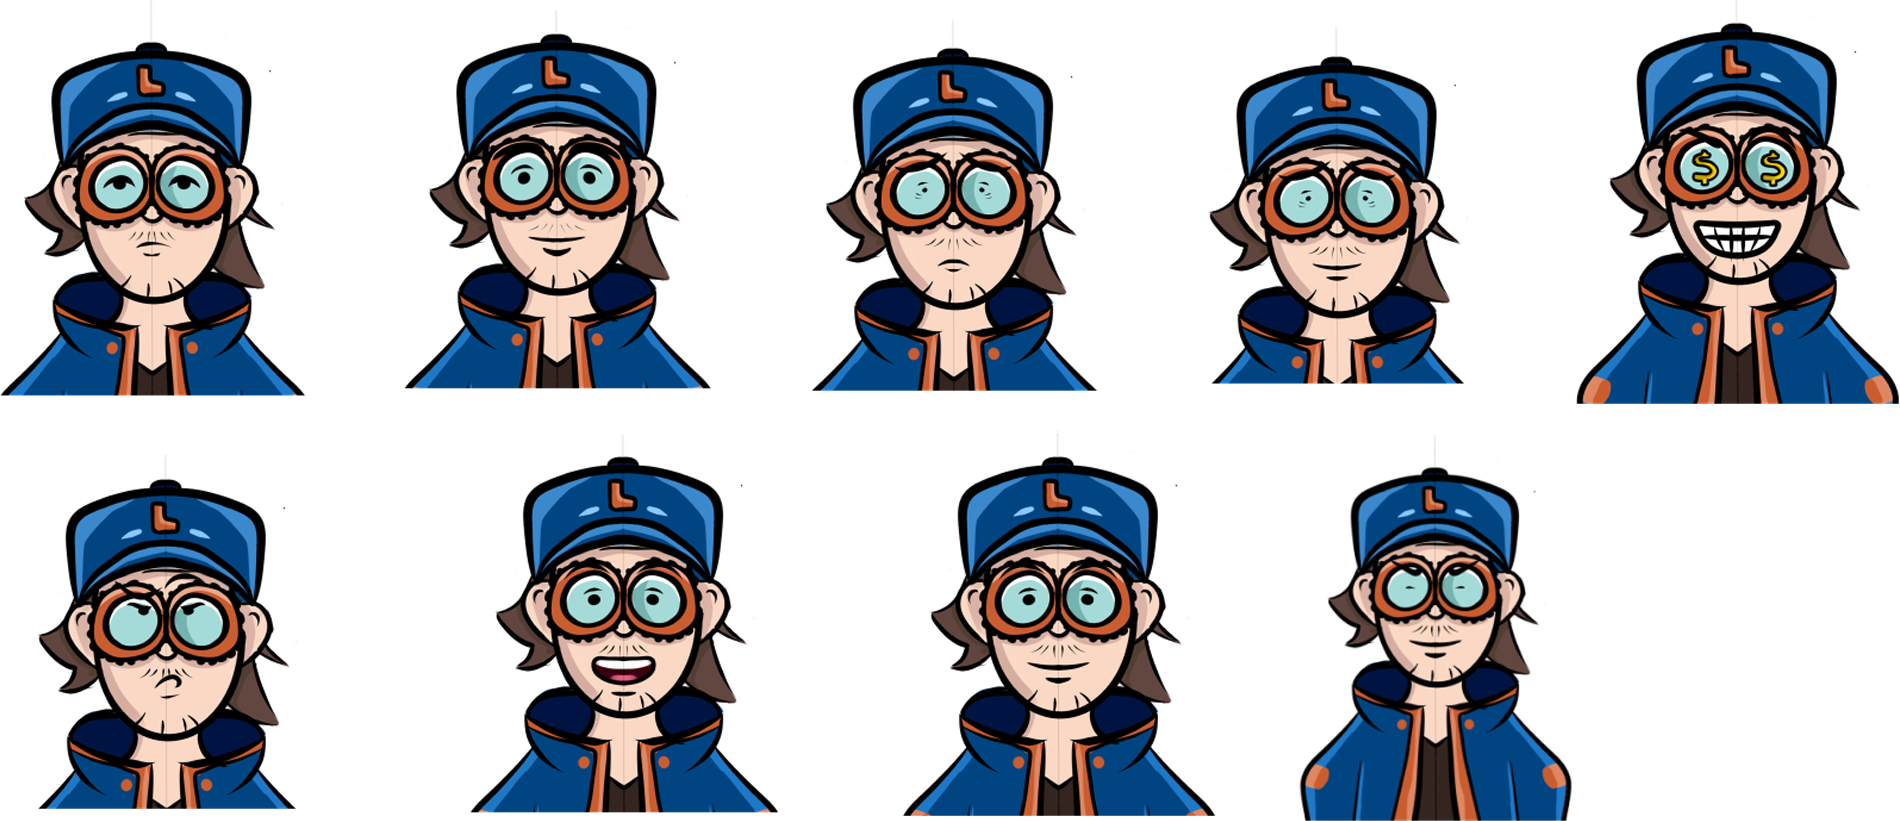
\includegraphics[width=8cm]{spreadsheet.png}
            \caption{Arte de conceito das expressões}
        \end{figure}
        
        O \emph{Pygame} foi a ferramenta para unir todos os elementos. Com os desenhos
        em mãos, fizemos a composição dos elementos na tela além de juntar os
        outros módulos (reconhecimento de voz e classificador% e pyaudio
        ). Iremos
        nos abster dos detalhes da arquitetura do front-end por não ser o foco
        do projeto.
        
        
        
    \subsection{Construção do Modelo}
    	% Conteúdos do notebook, não esquece dos prints tbm.
        A respeito da construção do modelo, como é detalhada por \emph{Jonathas dos Santos}
        e \emph{Lucas V.~de Lima} em seu documento
        especializado\cite{criacao-modelo}, foi feita com base no conjunto de
        dados \emph{Wikitext-2} a criação de um modelo de classificação
        genérico, sendo feito então um \emph{ajuste fino} com nossos próprios
        dados para a classificação em: Saudação, Despedida, Ordem de Compra,
        Ordem de Reembolso ou Listagem. 

        \begin{figure}[!h]
            \center
            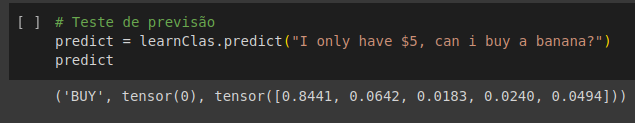
\includegraphics[height=1.5cm]{buyingBanana.png} \\
            \caption{\small{Teste do classificador}}
        \end{figure}
    	
    \subsection{Preparação dos Dados}
    	% Tudo pelo GPT
        Foi utilizado do ChatGPT para a geração de todos os dados do ajuste
        fino. Fizemos uma engenharia de prompt, onde demos as instruções para
        a IA gerar pacotes de 50 ou 100 frases simulando um cliente interagindo
        com o feirante. Demos sugestões de diversos cenários que ele deveria
        simular para, dessa forma, construirmos um conjunto de dados mais
        diverso possível. Segue link para uma das 
        \href{https://chat.openai.com/share/895c5da7-b209-4242-bace-1ce46108af37}{conversas
        de coleta de dados.}

        Um problema encontrado com essa abordagem foi a repetição de certos
        padrões que o Chat gerou. Para contorná-lo, fomos balizando a IA para
        deixar a amostra de dados menos viciada possível por meio de sugestões
        do tipo ``Faltou um inglês mais formal"  ou ``Repita menos a expressão
        Farewell...".

        \begin{figure}[!h]
            \center
            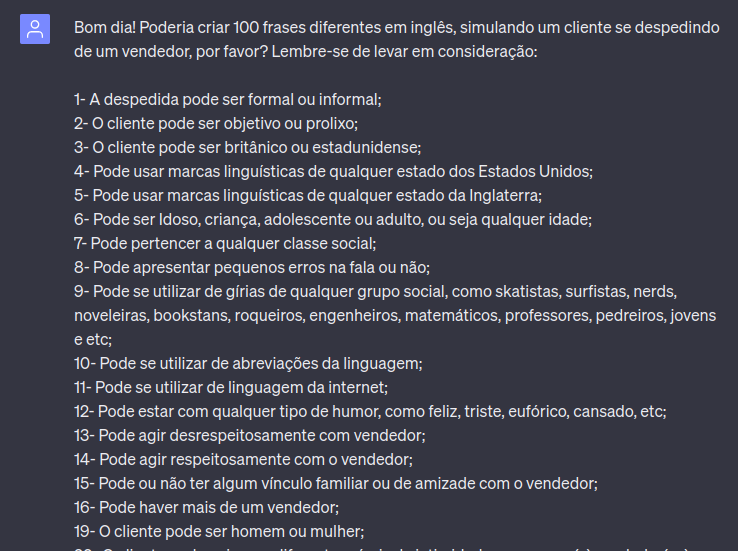
\includegraphics[width=8cm]{Dados2.png} \\
            \caption{\small{Pedido para geração de despedidas}}
        \end{figure}
        
    	
    \section{Conclusões}
        O projeto, mesmo ainda incompleto, foi muito gratificante de ser feito,
        dedicamos inúmeras horas e adquirimos diversas novas experiências e
        habilidades. Aprendemos tanto habilidades mais técnicas, como a criação
        de um modelo de NLP, prática com threads, engenharia de prompt e desenvolvimento do front-end,
        quanto habilidades mais sociais, como trabalho em equipe entre nós,
        buscar ajuda a colegas de outros cursos \footnote{Conversamos com um
        amigo de longa data que está fazendo graduação em IA na UFG, com o
        irmão de uma amiga sobre dicas de como prosseguir com o projeto e com o
        trio que fez um projeto de NLP na matéria de LIA, além da
        ajuda do artista, primo do Lucas.}, a importância de se ter um
        ``testador" para encontrar bugs no projeto \footnote{Percebemos, ao
        chamar uma pessoa externa ao projeto, que havia diversas falhas que nós,
        desenvolvedores, não iriamos encontrar sozinhos, pois estávamos com a
        mente limitada ao projeto.}. Foi uma bela oportunidade de nos
        esforçarmos para produzir algo interessante\footnote{Além da matéria de
        LIA, este documento é também nosso projeto final da matéria ``Editoração
        Acadêmica Básica com \LaTeX", onde tivemos a oportunidade de fazer um
        documento bem feito e apresentável, para facilitar a ilustração das
        ideias, por meio dos recursos que o \LaTeX{} oferece. Isso certamente
        nos auxiliará a escrever artigos no futuro.}. O projeto ainda
        está em desenvolvimento e temos uma lista de \emph{features} que
        gostaríamos de adicionar.

        


    \begin{thebibliography}{9}
        \bibitem{criacao-modelo} Jonathas dos Santos, Lucas V.~de Lima: \emph{Treinamento
            de Modelo de Processamento de Linguagem Natural para Classificação
            de Interações em Loja Virtual} (2023).
    \end{thebibliography}




        
\end{document}
